\section{Corrections for the Significance Adjustment in~\cite{zehlike2017fair}. }
\label{sec:adjustment-binomial}
%
In this section we describe extensions for the significance adjustment from~\cite{zehlike2017fair}.
%
We also provide a correction of the procedure which did not work for very small $k$ and $\alpha$. 

For binomial distributions, i.e. where only one protected and one non-protected group is present, the inverse CDF can be stored as a simple table, which we compute using Algorithm~\ref{alg:constructMTable}. 
%
Analogous to the multinomial case, we will call such a table \textit{mTable}.
%
Table~\ref{tbl:ranked_group_fairness_table} shows an example of such a pre-computed table with different $ k $ and $ p $, using $\alpha=0.1$.
%
For instance, for $p=0.5$ we see that at least 1 candidate from the protected group is needed in the top 4 positions, and 2 protected candidates in the top 7 positions.
\begin{algorithm}[h]
	\caption{Algorithm \algoMtable computes the data structure to efficiently verify or construct a ranking that satisfies binomial ranked group fairness.}
	\label{alg:constructMTable}
	\small
	\AlgInput{$k$, the size of the ranking to produce; $p$, the expected proportion of protected elements; $\alphaadj$, the significance for each individual test.}
	\AlgOutput{$ \mtable $: A list that contains the minimum number of protected candidates required at each position of a ranking of size $k$.}
	$\mtable \leftarrow [k]$ \AlgComment{list of size $k$} 
	\For{$i \leftarrow 1$ \KwTo $k$}{
		$\mtable[i] \leftarrow F^{-1}(i,p,\alphaadj)$ \AlgComment{the inverse binomial cdf}
	}
	\Return{$ \mtable $ }
\end{algorithm}

\begin{table}[h!]
	\small\begin{tabular}{r|cccccccccccc}
		\diaghead{some text}%
		{p}{k}&
		% & \multicolumn{10}{c}{k} \\
		1 & 2 & 3 & 4 & 5 & 6 & 7 & 8 & 9 & 10 & 11 & 12 \\ \midrule
		0.1      & 0 & 0 & 0 & 0 & 0 & 0 & 0 & 0 & 0 & 0  &  0 &  0 \\
		0.2      & 0 & 0 & 0 & 0 & 0 & 0 & 0 & 0 & 0 & 0  &  1 &  1 \\
		0.3      & 0 & 0 & 0 & 0 & 0 & 0 & 1 & 1 & 1 & 1  &  1 &  2 \\
		0.4      & 0 & 0 & 0 & 0 & 1 & 1 & 1 & 1 & 2 & 2  &  2 &  3 \\
		0.5      & 0 & 0 & 0 & 1 & 1 & 1 & 2 & 2 & 3 & 3  &  3 &  4 \\
		0.6      & 0 & 0 & 1 & 1 & 2 & 2 & 3 & 3 & 4 & 4  &  5 &  5 \\
		0.7      & 0 & 1 & 1 & 2 & 2 & 3 & 3 & 4 & 5 & 5  &  6 &  6 \\
		\bottomrule
	\end{tabular}
	\caption{Example values of $m_{\alpha,p}(k)$, the minimum number of candidates in the protected group that must appear in the top $k$ positions to pass the ranked group fairness criteria with $\alpha=0.1$ in a binomial setting.}
	\label{tbl:ranked_group_fairness_table}
\end{table}

Figure~\ref{fig:why-adjustment-is-needed-binomial} shows that we need a correction for $\alpha$ also in the binomial case (note that the scale is logarithmic).
%
In the following, we show that the special case of having only one protected group offers new possibilities for verifying ranked group fairness. 
%
A key improvement is that in the binomial setting we can calculate the exact failure probability $\failprob$ (i.e. a fair ranking gets rejected by the ranked group fairness test), which results in a much more efficient binary search for $\alphaadj$. 
%
Remember that in we had to estimate this probability for mTrees (see Section~\ref{sec:model-adjustment}) using an experimental procedure. 
%
First we introduce the necessary notation for the binomial case and describe how we calculate the exact $\failprob$.
%
Then we show that we can divide the continuum of possible $\alpha$ values in discrete parts in order to be able to apply efficient binary search for the most accurate $\alphaadj$.
%
Last we analyze the complexity of the proposed algorithms.
%This figure is generated by simulation, generating rankings using the process described above and showing the probability of those rankings being rejected by our ranked group fairness test with $\alphaadj=0.1$.
%
%The figure suggests that depending on $k$ we would need to change the value of $\alpha$ if we want to achieve a rejection rate of $0.1$.


\begin{figure}[h]
	\centering
	{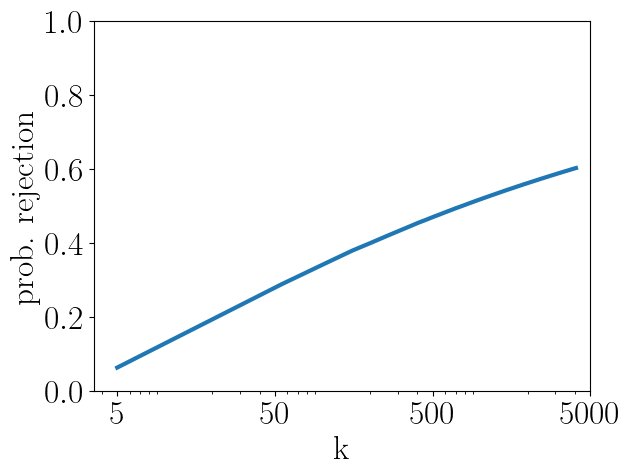
\includegraphics[width=.48\textwidth]{pics/failProbPlotBinom.png}}
	\caption{
		Probability that a fair ranking created by a Bernoulli process with $p=0.5$ fails the ranked group fairness test.\label{fig:why-adjustment-is-needed-binomial}
		%
		Experiments on data generated by a simulation, showing the need for multiple tests correction.
		%
		The data has: one protected group, with a ranking created by  a Bernoulli process (Fig.~\ref{fig:why-adjustment-is-needed-binomial}); and two protected groups, with a ranking created by a multinomial process (Fig.~\ref{fig:why-adjustment-is-needed-multinomial}).
		%
		Rankings should have been rejected as unfair at a rate $\alpha = 0.1$.
		%
		However, we see that the rejection probability increases with $k$.
		%
		Note the scale of $k$ is logarithmic.}
	\label{fig:need-for-model-adjustment}
\end{figure}

\subsection{Success Probability for One Protected Group}\label{subsubsec:adjustment-binomial}

The probability $\successprob$ that a fair ranking, created by the process of~\citet{yang2016measuring}, passes the ranked group fairness test (i.e. the success probability) with parameters $(p,\alpha)$ can be computed as follows:
%
Let $m(k) = m_{\alpha,p}(k) = F^{-1}(k,p,\alpha)$ be the number of protected elements required up to position $k$.
%
Let $\minv(i) = k$ s.t. $m(k) = i$ be the position at which $i$ protected elements are required.
%
Let $b(i) = \minv(i) - \minv(i-1)$ (with $\minv(0) = 0$) be the size of a ``block,'' that is, the gap between one increase and the next in $m(\cdot)$.
%
We call the $k$-dimensional vector $(m(1), m(2), \ldots , m(k))$ a \emph{mTable}.
%
An example is shown on Table~\ref{tbl:05:example_blocks}.
%
\begin{table}[b!]
	\centering
	\begin{tabular}{cccccccccccccc}\toprule
		$k$    & 1 & 2 & 3 & \textbf{{4}} & 5 & 6 & \textbf{7} & 8 & \textbf{9} & 10 & 11 & \textbf{12} \\
		\midrule
		$m(k)$ & 0 & 0 & 0 & \multicolumn{1}{c|}{1} & 1 & 1 & \multicolumn{1}{c|}{2} & 2 & \multicolumn{1}{c|}{3} & 3  & 3  & \multicolumn{1}{c}{4}\\
		Inverse   & \multicolumn{4}{c|}{$\minv(1)=4$}
		& \multicolumn{3}{c|}{$\minv(2)=7$}
		& \multicolumn{2}{c|}{$\minv(3)=9$}
		& \multicolumn{3}{c}{$\minv(4)=12$}\\
		Blocks       & \multicolumn{4}{c|}{$b(1)=4$}
		& \multicolumn{3}{c|}{$b(2)=3$}
		& \multicolumn{2}{c|}{$b(3)=2$}
		& \multicolumn{3}{c}{$b(4)=3$}\\
		\bottomrule
	\end{tabular}
	\caption[Example of different block sizes]{Example of $m(\cdot)$, $\minv(\cdot)$, and $b(\cdot)$ for $p=0.5, \alpha=0.1$.}
	\label{tbl:05:example_blocks}
\end{table}

\noindent Furthermore let
\begin{equation}
	\label{eq:05:combinations}
	I_{m(k)} = \{ v = (i_1, i_2, \ldots, i_{m(k)}): \forall \ell' \in \lbrace 1,\ldots,m(k) -1 \rbrace, 0 \le i_{\ell'} \le b(\ell') \wedge \sum_{j=1}^{\ell'} i_j \ge \ell' \}
\end{equation}
%
represent all possible ways in which a fair ranking\footnote{Note that we do not consider rankings of size 0, which always pass the test.} generated by the method of \citet{yang2016measuring} can pass the ranked group fairness test, with $i_j$ corresponding to the number of protected elements in block $j \; (\text{with } 1 \le j \le k)$.
%
As an example consider again Table~\ref{tbl:05:example_blocks}: the first block contains four positions, i.e. $b(1)=4$ and this block passes the ranked group fairness test, if it contains at least one protected candidate, hence $i_1 \in \{1, 2, 3, 4\}$.
%
The probability of considering a ranking of $k$ elements (i.e. $m(k)$ blocks) unfair, is:
\begin{equation}
	\label{eq:05:failureProb}
	\failprob = 1 - \successprob = 1 - \sum_{v \in I_{m(k)}} \prod_{j=1}^{m(k)} f(v_j; b(j), p)
\end{equation}
%
\noindent where $f(x;b(j),p) = Pr(X = x)$ is the probability density function (PDF) of a binomially distributed variable $X \sim Bin(b(j), p)$.
%
However, if calculated naively this expression is intractable because of the large number of combinations in $I_{m(k)}$.
%

\setlength{\textfloatsep}{2pt}% Remove \textfloatsep
\begin{algorithm}[t!]
	\caption{Algorithm \algoRecursive computes the probability, that a given mTable accepts a fair ranking (see right term of Eq.~\ref{eq:05:failureProb}).}
	\label{alg:05:successProb} % But whenever possible refer to this algo. by name not number
	\small
	\AlgInput{
		$\texttt{b[]}$ list of block lengths (Table~\ref{tbl:05:example_blocks}, 3rd line);\\ 
		$\texttt{maxProtected}$ the sum of all entries of $\texttt{b[]}$;\\
		$\texttt{currentBlockIndex}$ index of the current block; \\
		$\texttt{candidatesAssigned}$ number of protected candidates assigned for the current possible solution; \\
		$p$, the expected proportion of protected elements.}
	\AlgOutput{The probability of accepting a fair ranking.}
	
	\If{$\texttt{b[].length} = 0$}{
		\Return{$1$}
	}
	\tcp{we need to assign at least one protected candidate to each block}
	$\texttt{minNeededThisBlock} \leftarrow \texttt{currentBlockIndex} - \texttt{candidatesAssigned}$\\
	\tcp{if we already assigned enough candidates, minNeededThisBlock = 0 (termination condition for the recursion)}
	\If{$\texttt{minNeededThisBlock} < 0$}{
		$\texttt{minNeededThisBlock} \leftarrow 0$
	}
	$\texttt{maxPossibleThisBlock} \leftarrow \textit{argmin}(\texttt{b[0]}, \texttt{maxProtected})$ \\
	$\texttt{assignments} \leftarrow 0$ \\
	$\texttt{successProb} \leftarrow 0$ \\
	\tcp{sublist without the first entry of $\texttt{b[]}$}
	$\texttt{b\_new[]} \leftarrow \textit{sublist}(\texttt{b[]}, 1, \texttt{b[].length})$ \label{algoline:05:suffixes}\\
	$\texttt{itemsThisBlock} \leftarrow \texttt{minNeededThisBlock}$\\
	\While{$\texttt{itemsThisBlock} \leq \texttt{maxPossibleThisBlock}$}{
		$\texttt{remainingCandidates} \leftarrow \texttt{maxProtected} - \texttt{itemsThisBlock}$ \\
		$\texttt{candidatesAssigned} \leftarrow \texttt{candidatesAssigned} + \texttt{itemsThisBlock}$ \\
		\tcp{each recursion returns the success probability of \emph{all possible ways} to fairly rank protected candidates after this block}
		$\texttt{suffixSuccessProb} \leftarrow \textsc{\algoRecursive} ( $ \\ \pushline $ \texttt{remainingCandidates},\texttt{b\_new[]}, \texttt{currentBlockIndex} + 1,$ \\ $ \texttt{candidatesAssigned})$ 
		\label{algoline:05:recursion}\\
		\popline $\texttt{totalSuccessProb} \leftarrow \texttt{totalSuccessProb} \; + $ \\ \pushline $ \textsc{PDF}(\texttt{maxPossibleThisBlock}, \texttt{itemsThisBlock}, p) \; \cdot $ \\ $ \texttt{suffixSuccessProb}$ \label{algoline:05:pdf}\\
		\popline $\texttt{itemsThisBlock} \leftarrow \texttt{itemsThisBlock} + 1$\\
	}
	\Return{probability of accepting a fair ranking: $\texttt{totalSuccessProb}$ }
\end{algorithm}
We therefore propose a dynamic programming method, Algorithm~\ref{alg:05:successProb}, which computes the probability that a fair ranking passes the ranked group fairness test (i.e. the right term of Equation~\ref{eq:05:failureProb}) \emph{recursively}.
%
Note that because of the combinatorial complexity of the problem a \emph{simple closed-form expression} to compute $\failprob$ is unlikely to exist.
%With this algorithm however, we have to account for an important pitfall: we may choose a combination of $k, p, \alpha$ where the last block ``reaches beyond'' $k$.
%
%Consider again Table~\ref{tbl:05:example_blocks} with $k=8, \minpro$p=$0.5, \alpha=0.1$: the second block reaches until position 7, while the third block reaches until position 9.
%
%If we cut off the mTable at $k=8$ to adjust the significance level, the last block reaches beyond $k$ which is to position 9.
%
%\meike{Inwiefern macht der neue Algorithmus das Problem mit aufgebrochenen Blöcken besser?}
%To account for that t
The algorithm breaks the vector $v = (i_1, i_2, \ldots ,i_{\ell})$ of Equation~\ref{eq:05:combinations} into a \textit{prefix} and a \textit{suffix} (Alg.~\ref{alg:05:successProb}, Line~\ref{algoline:05:suffixes}).
%
We call $i_1$ the \textit{prefix} of $(i_2, \ldots, i_{\ell})$, and $(i_2, \ldots, i_{\ell})$ the \textit{suffix} of $i_1$.
%
The algorithm starts with a prefix and calculates all possible suffixes, that pass the ranked group fairness test, recursively (Line~\ref{algoline:05:recursion}).
%
Consider the following example: for the first prefix $i_1 = 1$ the algorithm computes all possible suffixes, where we rank exactly one protected candidate in the first block.
%
For this prefix $i_1$, combined with each possible suffix $v \setminus i_1$, we calculate the success probability $\prod_{j=1}^{m(k)} f(v_j; b(j), p)$ for each instance of $v$ (Line~\ref{algoline:05:pdf}).
%
In the next recursion level we start with a new prefix, let us say $i_1=1, i_2 =1$.
%
The algorithm computes all possible suffixes, i.e. all rankings where we rank exactly one protected candidates in the first block and one protected candidate in the second block.
%
Then it computes the respective success probabilities.
%
This procedure continues for $m(k)$ iterations.
%
After that the whole program starts again with $i_1=2$ and is repeated until the maximum number of protected candidates is reached, in our case $b(1)=4$.
%
All intermediate success probabilities are added up (Line~\ref{algoline:05:pdf}) to the total success probability (see Eq.~\ref{eq:05:failureProb}) of the mTable that was created given $k, p, \alpha$.

Note that there are at most $\prod_{j=1}^{m(k)}b(j)$ possible combinations to distribute the protected candidates within the blocks.
%
Furthermore many $v \in I_{m(k)}$ share the same prefix and hence have the same probability density value for these prefixes.
%
To reduce computation time the algorithm stores the binomial probability density value for each prefix in a hash map with the prefix as key and the respective pdf as value.
%
Thus the overall computational complexity becomes $O(\prod_{j=1}^{m(k)}b(j) \cdot O(\texttt{binomPDF}))$.

\subsection{Finding the Correct mTable}\label{subsec:finding-mtable}
We call an mTable \textit{correct} if it has an overall success probability of $\successprob = 1-\alpha$. 
However, given parameters $k,p,\alpha$, $\successprob$ will be greater or equal to $1-\alpha$. Thus, we need a corrected $\alphaadj \leq \alpha$ in order to compute the correct mTable. Unfortunately there is no way to compute $\alphaadj$ directly, which is why we have to search for the correct mTable, hence $\alphaadj$. 
We propose Algorithm~\ref{alg:05:binarySearch} that takes  parameters $k, p, \alphaadj$ as input and returns the correct mTable and $\alphaadj$.
%
%We use Algorithm~\ref{alg:05:successProb} to determine the adjusted significance level $\alphaadj$ for the ranked group fairness test, such that the overall acceptance probability for the mTable with parameters $k, p, \alphaadj$ becomes $1-\alpha$.
%
It sequentially creates mTables (recall that these are $k$-dimensional vectors of the form $(m(1), m(2), \ldots , m(k))$) for different values of $\alphaadj$, and then calls Algorithm~\ref{alg:05:successProb} to calculate their success probability until it finds the correct mTable with overall failure probability $\failprob = \alpha$ . 
%
Our goal is to use binary search to select possible candidates for $\alphaadj$ systematically.

%\note[ChaTo]{Perhaps the definition of the mass of an mTable can wait a few more paragraphs, until you need it.}
However, to be able to do binary search, we need a discrete measure for the $\alpha$-space to search on, otherwise the search would never stop. Specifically, we could never be sure if we found the mTable with the minimum difference of $\successprob$ to $1-\alpha$. A binary search would further and further divide an interval between two $\alpha$ values. The only chance to verify that we do not have to search further is by comparing the resulting mTables of different $\alpha$ values. We will see, that we can do that by comparing the sum of the entries in the mTable and that there exist only a limited number of them.
%
Furthermore, to reduce complexity we only want to consider mTables with certain properties, which we define in the following paragraph. 
%
A $k$-dimensional vector (e.g. $(0,0,1,2,3)$) has to have two properties in order to constitute a mTable, rather than just a vector of natural numbers: it has to be \emph{valid} and \emph{legal}.
%
\begin{definition}[Valid mTable]
	\label{def:05:valid-mtable}
	The $\text{mTable}_{p,k,\alpha}=(m(1) , m(2) , \ldots , m(k))$ is \emph{valid} if and only if, $m(i) \leq m(j)$ for all $i,j \in \lbrace 0, \ldots, k \rbrace$ with $i < j$ and $m(i)=n \Rightarrow m(i+1) \leq n+1$.
\end{definition}
\noindent It is easy to see that many valid mTables exist.
%
They correspond to all $k$-dimensional arrays with integers monotonically increasing by array indices.
%
However we only want to consider those valid mTables for our ranked group fairness test that have been created by the statistical process in~\citet{yang2016measuring}.
%
We call these \textit{legal mTables}.
%
\begin{definition}[Legal mTable]
	\label{def:05:legal-mtable}
	A $\text{mTable}_{p,\alpha,k}$ is \textit{legal} if and only if there exists a $p,k,\alpha$ such that
	$\texttt{constructMTable}(p,k,\alpha)=\text{mTable}_{p,\alpha,k}$.
\end{definition}
%
Definition \ref{def:05:legal-mtable} restricts the space of k-dimensional arrays to those which are computed by a specific function. Since the mTable is a datastructure that should represent the minimum proportions required for a specific dice roll, we have to define $\texttt{constructMTable}$ such that it represents this process. Otherwise we could think of various ways to define processes to compute possible mTables.
\begin{definition}[constructMTable]
	\label{def:05:construct-mtable-single-test}
	For $p\in [0,1], k \in \mathbb{N}, \alpha \in [0,1]$ we define a function to construct a mTable from input parameters $p, k, \alpha$ according to \cite{yang2016measuring}.
	
	\noindent$\texttt{constructMTable} : \\ (0,1) \times \mathbb{N} \times [0,1] \longrightarrow \lbrace (m(1) ,\ldots, m(k)): m(i) = F^{-1}(i,p,\alpha), \, i = \{1,\ldots,k\}\rbrace$ \\
	with $\texttt{constructMTable}(p,k,\alpha)=\text{mTable}_{p,k,\alpha}$.
\end{definition}
%
\begin{lemma}
	\label{lemma:05:legal-valid-mtable}
	If a mTable is legal, it is also valid.
\end{lemma}
%
\noindent Lemma \ref{lemma:05:legal-valid-mtable} follows directly by construction.
%
Now we need a discrete partition of the continuous $\alpha$ space, that is a discrete measure that corresponds to exactly one legal mTable for a given set of parameters $k,p,\alpha$. 
%
We call this measure the \emph{mass} of a mTable.
%The definition of a legal mTable together with its corresponding mass enables us to perform a binary search, which helps us to find $\alphaadj$ and hence the correct mTable with an overall failure probability of $\alpha$.
%
%Note that for any value of $\alpha$ there exists exactly one \emph{legal} mTable.
%
%However, the opposite is not true: as $\alpha$ is a real number from the interval $[0, 1]$, the same mTable can be created using different (but very similar) values of $\alpha$.
%
%Thus without a discrete measure for a mTable we do not know when to stop searching, which is why we introduce the \emph{mass of a mTable}.
%
\begin{definition}[Mass of a mTable]
	\label{def:05:Mass of a MTable}
	For $\text{mTable}_{p,k,\alpha}=(m(1) , m(2) , \ldots , m(k))$ we call\\
	$L_1(\text{mTable}_{p,k,\alpha})=\sum_{i=1}^k m(i)$ the \textit{mass of $\text{mTable}_{p,\alpha,k}$}.
\end{definition}
%
In the following we relate the continuous $\alpha$-space to the discrete mass of a mTable.
%
\begin{lemma}
	\label{lemma:05:non-decreasing-with-alpha-mtable}
	Every $\text{mTable}_{p,k,\alpha}=\texttt{constructMTable}(p,k,\alpha)=(m(1) , m(2) , \ldots , m(k))$ is non-decreasing with $\alpha$. This means that
	$\texttt{constructMTable}(p,k,\alpha - \epsilon) = (m(1)' , m(2)' , \ldots , m(k)')$ will result in $m(i)' \leq m(i)$ for $i=1,\ldots,k$ and $\epsilon > 0$.
\end{lemma}
\begin{proof}
\label{proof:05:non-decreasing-with-alpha-mtable}
Every entry $m(i)$ for $i=1,\ldots,k$ is computed by line 3 of Algorithm~\ref{alg:constructMTable}, i.e. every entry is the inverse binomial cdf $F^{-1}(i,p,\alphaadj)$. In other words $m(i)$ is the smallest integer such that\\
\begin{equation}
\alphaadj \leq \sum_{j=0}^{m(i)}\binom{i}{j}p^i (1-p)^{i-j} = F^{-1}(i,p,\alphaadj)
\end{equation}
The following equivalence holds:
\begin{equation}\label{eq:smaller m}
\alphaadj - \epsilon \leq \sum_{j=0}^{m'(i)}\binom{i}{j}p^i (1-p)^{i-j} = F^{-1}(i,p,\alphaadj-\epsilon)
	\Leftrightarrow \alphaadj \leq \sum_{j=0}^{m'(i)}\binom{i}{j}p^i (1-p)^{i-j} + \epsilon
\end{equation}
Now suppose that $m'(i) > m(i)$ which contradicts lemma \ref{lemma:05:non-decreasing-with-alpha-mtable}. 
%
Then it is that
\[m'(i)>m(i) \Rightarrow \sum_{j=0}^{m'(i)}\binom{i}{j}p^i (1-p)^{i-j} \geq \sum_{j=0}^{m(i)}\binom{i}{j}p^i (1-p)^{i-j}\]
because $\binom{i}{j}p^i (1-p)^{i-j} \geq 0 \; \forall i,j,p$. It follows for $\epsilon >0$ that
\begin{equation}
\alphaadj \leq \sum_{j=0}^{m(i)}\binom{i}{j}p^i (1-p)^{i-j} + \epsilon \leq \sum_{j=0}^{m'(i)}\binom{i}{j}p^i (1-p)^{i-j} + \epsilon
\end{equation}
But then $m'(i)\neq F^{-1}(i,p,\alphaadj-\epsilon)$ because $m(i)$ would be the smaller integer that satisfies Equation~\ref{eq:smaller m}. Thus it has to be that $m'(i)\leq m(i)$.
\end{proof}
%
\noindent This property shows that, if we reduce $\alpha$ in our binary search, the mass of the corresponding mTable is also reduced or stays the same.
%
It very usefully implies a criterion to stop the binary search: namely we stop the calculation when the mass of the mTable at the left search boundary equals the right search boundary.
%
Of course this only works if there exists exactly one legal mTable for each mass, which we proof in the following.
\begin{theorem}
	\label{theorem:05:mtable-mass-injection}
	For fix $p,k$ there exists exactly one legal mTable for each mass $L_1\in \lbrace 1,\ldots,k \rbrace$.
\end{theorem}
%
\begin{proof}
	\label{proof:05:mtable-mass-injection}
	We prove this by contradiction: Let $MT_{p,k,\alpha_1}$ and $MT'_{p,k, \alpha_2}$ be two different mTables with $L_1(MT_{p,k,\alpha_1 }) = L_1(MT'_{p,k,\alpha_2})$.\\
	%
	If both are legal then it applies that $\texttt{constructMTable}(p,\alpha_1 ,k)=MT_{p,\alpha_1 ,k}$
	and \\ $\texttt{constructMTable}(p,\alpha_2 ,k)=MT'_{p,\alpha_2 ,k}$.
	%
	Because $MT_{p,k,\alpha_1} \neq MT'_{p,k,\alpha_2}$, without loss of generality entries $m(i), m(i)' , m(j) , m(j)'$ exist in each table, such that $|m(i) - m(i)'| = |m(j) - m(j)'|$ while at the same time $m(i) > m(i)'$ , $m(j) < m(j)'$ for $i<j, i,j \in \lbrace 1, \ldots , k \rbrace$.
	%
	(Think of it as the two entries in each table "evening out", such that both tables have the same mass.)\\
	%
	If $\alpha_1 > \alpha_2$, then the statement $m(j)' > m(j)$ violates Lemma~\ref{lemma:05:non-decreasing-with-alpha-mtable}.
	%
	If $\alpha_2 > \alpha_1$, then the statement $m(i) > m(i)'$ also violates Lemma~\ref{lemma:05:non-decreasing-with-alpha-mtable}.
	%
	The only possibility left is hence that $\alpha_1 = \alpha_2$, which contradicts $MT \neq MT'$, as both are created using function \texttt{constructMTable}.
\end{proof}
%
With these mathematical properties we can perform a binary search on the continuous $\alpha$-space to find the corrected significance level $\alphaadj$.
%
This corrected significance is used to compute a final mTable with an overall failure probability $\failprob = \alpha$.
\begin{algorithm}[t!]
	\caption{Algorithm \algoBinomBinary calculates the corrected significance level $\alpha_c$ and the mTable $m_{\alpha_c , k, p)}$ with an overall probability $\alpha$ of rejecting a fair ranking.}
	\label{alg:05:binarySearch} % But whenever possible refer to this algo. by name not number
	\footnotesize
	\AlgInput{$k$, the size of the ranking to produce; $p$, the expected proportion of protected elements; $\alpha$, the desired significance level.}
	\AlgOutput{$\alphaadj$ the adjusted significance level; \texttt{m\_{adjusted}} the adjusted mTable}
	\AlgComment{initialize all needed variables}
	\texttt{aMin $\leftarrow$ 0};
	\texttt{aMax $\leftarrow \alpha$ };
	\texttt{aMid} $\leftarrow \frac{(\texttt{aMin + aMax})}{2}$ \\
	\texttt{m\_min} $\leftarrow$ \texttt{constructMTable(k,p,aMin)}; 
	\texttt{m\_max} $\leftarrow$ \texttt{constructMTable(k,p,aMax)}; \\
	\texttt{m\_mid} $\leftarrow$ \texttt{constructMTable(k,p,aMid)} \\
	\texttt{maxMass} $\leftarrow$ \texttt{m\_max.getMass()};
	\texttt{minMass} $\leftarrow$ \texttt{m\_min.getMass()};
	\texttt{midMass} $\leftarrow$ \texttt{m\_mid.getMass()}\\
	
	\While{\texttt{minMass} $<$ \texttt{maxMass} AND \texttt{m\_mid.getFailProb()} $\neq \alpha$ }{
		\If{\texttt{m\_mid.getFailProb()} $< \alpha$}{
			\texttt{aMin} $\leftarrow$ \texttt{aMid}
			\texttt{m\_min} $\leftarrow$ \texttt{constructMTable(k,p,aMin)} \\
		}
		\If{\texttt{m\_mid.getFailProb()} $> \alpha$}{
			\texttt{aMax} $\leftarrow$ \texttt{aMid} \\
			\texttt{m\_max} $\leftarrow$ \texttt{constructMTable(k,p,aMax)} \\
		}
		\texttt{aMid} $\leftarrow \frac{(\texttt{aMin + aMax})}{2}$ \\
		\tcp{stop criteria if midMass equals maxMass or midMass equals minMass}
		\If{\texttt{maxMass - minMass == 1}}{
			\texttt{minDiff} $\leftarrow |$\texttt{m\_min.getFailProb() - }$\alpha|$ \\
			\texttt{maxDiff} $\leftarrow |$\texttt{m\_max.getFailProb() - }$\alpha|$ \\
			\tcp{return the $\alpha_c$ which has the lowest difference from the desired significance}			
			\If{\texttt{minDiff} $<$ \texttt{maxDiff}}{
				\Return{\texttt{aMin, m\_min}}
			}
			\Else{
				\Return{\texttt{aMax, m\_max}}
			}
		}
		\tcp{stop criteria if midMaxx is exactly the mass between minMass and maxMass}
		\If{\texttt{maxMass - midMass == 1} AND \texttt{midMass - minMass == 1}}{
			\texttt{minDiff} $\leftarrow |$\texttt{m\_min.getFailProb() - }$\alpha|$ \\
			\texttt{maxDiff} $\leftarrow |$\texttt{m\_max.getFailProb() - }$\alpha|$ \\
			\texttt{midDiff} $\leftarrow |$\texttt{m\_mid.getFailProb() - }$\alpha|$ \\
			\tcp{return the $\alpha_c$ which has the lowest difference from the desired significance}			
			\If{\texttt{midDiff} $\leq$ \texttt{maxDiff} AND \texttt{midDiff} $\leq$ \texttt{minDiff}}{
				\Return{\texttt{aMid, m\_mid}}
			}
			\If{\texttt{minDiff} $\leq$ \texttt{midDiff} AND \texttt{minDiff} $\leq$ \texttt{maxDiff}}{
				\Return{\texttt{aMin, m\_min}}
			}
			\Else{
				\Return{\texttt{aMax, m\_max}}
			}
		}
	}
	\Return{\texttt{aMid, m\_mid}}
\end{algorithm}

\subsection{Complexity in the Binomial Case} 
\begin{table}[t!]
	\caption{Time complexity for all algorithms for one protected group without pre-computed results.\label{tbl:time-space-binom}}
	\vspace{-4mm}
	\scalebox{0.75}{
		\begin{tabular}{lll}
			\toprule
			\textbf{Algorithm} & \textbf{Time Complexity} & \textbf{Space Complexity}\\
			\midrule
			\rowcolor[HTML]{C0C0C0}
			\algoMtable & $\mathcal{O}(k) \cdot \mathcal{O}(F^{-1}(p,k,\alpha))$ & $\mathcal{O}(k)$ \\
			\algoRecursive & $\mathcal{O}(\texttt{\algoMtable}) + \mathcal{O}(\prod_{j=1}^{m(k)}b(j) \cdot O(\texttt{binomPDF}))$ & $\mathcal{O}(k)$ \\
			\rowcolor[HTML]{C0C0C0}
			\algoBinomBinary & $\mathcal{O}(\log{}k) \cdot (\mathcal{O}(\texttt{\algoRecursive}))$ & $\mathcal{O}(k)$  \\
			\bottomrule
		\end{tabular}
	}
\end{table}

In order to estimate the complexity of the whole procedure (and hence understand its computational feasibility), we need to know how many mTables exist for fix $k$ and $p$.
%
%\note[ChaTo]{@Tom: please check if the following sentence that I added is correct, I thought it would make this more understandable.}
This is the number of non-decreasing sequences of integers that end with a number smaller or equal to $k$ and have length $k$.
%
\begin{theorem}
	\label{theorem:05:number-of-mtables}
	The number of legal mTables for $k,p$ is less or equal to $\frac{k(k-1)}{2}$ .
\end{theorem}

\begin{proof}
	\label{proof:05:number-of-mtables}
	Given the proof of Theorem~\ref{theorem:05:mtable-mass-injection} we can count the number of legal mTables for fix $p,k$ as follows: The maximum mass of a legal mTable of length $k$ is by construction
	$L_1 ((m(1) = 1,m(2) = 2, \ldots, m(k) = k)) = \sum_{i=1}^k m(i) = \frac{k(k-1)}{2}$. 
	%
	Following definition~\ref{def:05:valid-mtable} the 	    entry $m(1)$ is the smallest entry or equal to all other entries. 
	%
	Furthermore, because this mTable is legal and following Definition~\ref{def:05:legal-mtable}, the mTable is a result of Algorithm~\ref{alg:constructMTable}. 
	%
	Thus $m(1) = F^{-1}(1,p,\alpha) \in \lbrace 0,1\rbrace$. In other words, $m(1)$ can only be $0$ or $1$.
	
	%
	In turn $m(2)$ can only be $2$, if $m(1)$ was $1$ (otherwise $m(2)<2$).
	%
	Accordingly, the minimum mass of a legal mTable is $L_1((m(1),m(2), \ldots, m(k))) = 0$, if all $m(i)=0$.
	%
	Following Lemma~\ref{lemma:05:non-decreasing-with-alpha-mtable}, we can create mTables with higher masses by increasing $\alpha$. 
	%
	Furthermore, following Theorem~\ref{theorem:05:mtable-mass-injection}, if a legal mTable exists for a given mass and parameters $k,p$, then this is the only existing legal mTable with that mass.
	%
	We know that there is a theoretical minimum mass for legal mTables ($L_1 =0$) which would occur, for example, if we set $\alpha = 0$ assuming $p<1$.
	%
	There also exists a theoretical maximum mass for legal mTables which is $\frac{k(k-1)}{2}$. 
	%
	At best, we can achieve every possible mass between those two to extremes. 
	%
	It follows that there are at most $\frac{k(k-1)}{2}$ masses for legal mTables of size $k$ for a fix~$p$.
\end{proof}
%
Table \ref{tbl:time-space-binom} shows space and time complexities for the algorithms of the binomial case. 
%
\subsubsection{\algoMtable complexity}\label{subsubsec:construct-mtable-complexity}
\algoMtable computes the inverse binomial cdf for k positions of the ranking and stores each of the computed values.
%
This leads to a time complexity of $\mathcal{O}(k) \cdot \mathcal{O}(inverseBinomialCDF(p,k,\alpha))$.  Assuming a constant time for the calculation of the binomial probability mass function, the time complexity of the implementation for the inverse binomial cdf which we used is in $\mathcal{O}(i^2)$ where $i$ is the position we calculate the inverse binomial cdf for.
%
Note that the complexity of the inverse binomial cdf is dependent on how accurate the computation is.
%
The space complexity is $\mathcal{O}(k)$ if we do not store any intermediate results for future calculations.
%
\subsubsection{\algoRecursive complexity}\label{subsubsec:success-prob-complexity}
The algorithm \algoRecursive has time complexity $\mathcal{O}(\prod_{j=1}^{m(k)}b(j) \cdot O(\texttt{binomPDF}))$ as explained in section \ref{subsubsec:adjustment-binomial}.
%
Before that we have to calculate the mTable and blocks $b$ which adds $\mathcal{O}(k) \cdot \mathcal{O}(F^{-1}(p,k,\alpha))$ and $\mathcal{O}(k)$ respectively to the complexity.
%
Overall we get $\mathcal{O}(k) \cdot \mathcal{O}(F^{-1}(p,k,\alpha)) + \mathcal{O}(\prod_{j=1}^{m(k)}b(j) \cdot O(\texttt{binomPDF}))$.
%
For the sake of readability we will write $\mathcal{O}($\algoMtable$) + \mathcal{O}(\prod_{j=1}^{m(k)}b(j) \cdot O(\texttt{binomPDF}))$.
%
The space complexity is $\mathcal{O}(k)$ for the maximum number of blocks plus $\mathcal{O}(k)$ for the stored probabilities at each position.
%
\subsubsection{\algoBinomBinary complexity}\label{subsubsec:binom-binary-complexity}
The binary search for $\alpha_c$ has a complexity of $\mathcal{O}(\log{}\frac{k(k-1)}{2}) = \mathcal{O}(\log{}k^2) = \mathcal{O}(\log{}k)$, because maximum $\frac{k(k-1)}{2}$ different valid mTables exist.
%
For each binary search step we need $\mathcal{O}(\mathcal{O}(k) \cdot \mathcal{O}(F^{-1}(p,k,\alpha)))$ to compute the new mTable as well as $\mathcal{O}(\prod_{j=1}^{m(k)}b(j) \cdot O(\texttt{binomPDF}))$ for its fail probability.
%
Overall we get $\mathcal{O}(\log{}k) \cdot (\mathcal{O}(\prod_{j=1}^{m(k)}b(j) \cdot O(\texttt{binomPDF})) + \mathcal{O}(\mathcal{O}(k) \cdot \mathcal{O}(F^{-1}(p,k,\alpha))))$, which we will write as $\mathcal{O}(\log{}k) \cdot (\mathcal{O}(\texttt{\algoRecursive}))$.
%
The space complexity is $\mathcal{O}(k)$ since we only store the three MTables with their respective fail probability.